\chapter{ Electromagnetic Transients }
\label{ch:etr}

The simulation and analysis of electromagnetic transients in basic electric circuits are essential to the study of power systems. Electromagnetic transient analysis software can help to determine overcurrent, overvoltage and other unwanted phenomena in power systems.  Since the 1970s, computer-aided algorithms have been developed to simulate a wide variety of conditions on complex circuits. 


\blockquote[\cite{martinez2015introduction}]{
Despite the powerful numerical techniques, simulation tools and graphical user interfaces currently
available, those involved in electromagnetic transients studies, sooner or later, face the limitations of
models available in transients packages, the lack of reliable data and conversion procedures for parameter
estimation or insufficient studies for validating models
}

Some of these simulation tools are well-known in industry and academia, such as ATP and EMTP. These two programs operate by creating a representation of the equivalent input circuit and obtaining the simulation results either by state space or nodal analysis. This work is focused on the latter approach.

\section{ Overview of Nodal Analysis }
\label{solutionalg}

Broadly studied at electromagnetic transients courses and firstly described by H. Dommel in \cite{dommel1969digital}, the nodal admittance matrix method is the base algorithm for programs like EMTP and ATP. This representation can deal with both single and multi-phase circuits containing resistors, capacitors, sources and a few other nonlinear elements as well as the discretization of the circuit differential equations through the trapezoidal integration method.


Figure \ref{transient1} illustrates a simple circuit and the continuous time domain first order differential equation and its solution for the current as function of time, considering the time constant (L/R) of the circuit.


\begin{figure}[H]
  \caption{Transient Analysis - Example Circuit}
  \centering
  \begin{minipage}[c]{0.59\linewidth}  
  %\subfloat{
    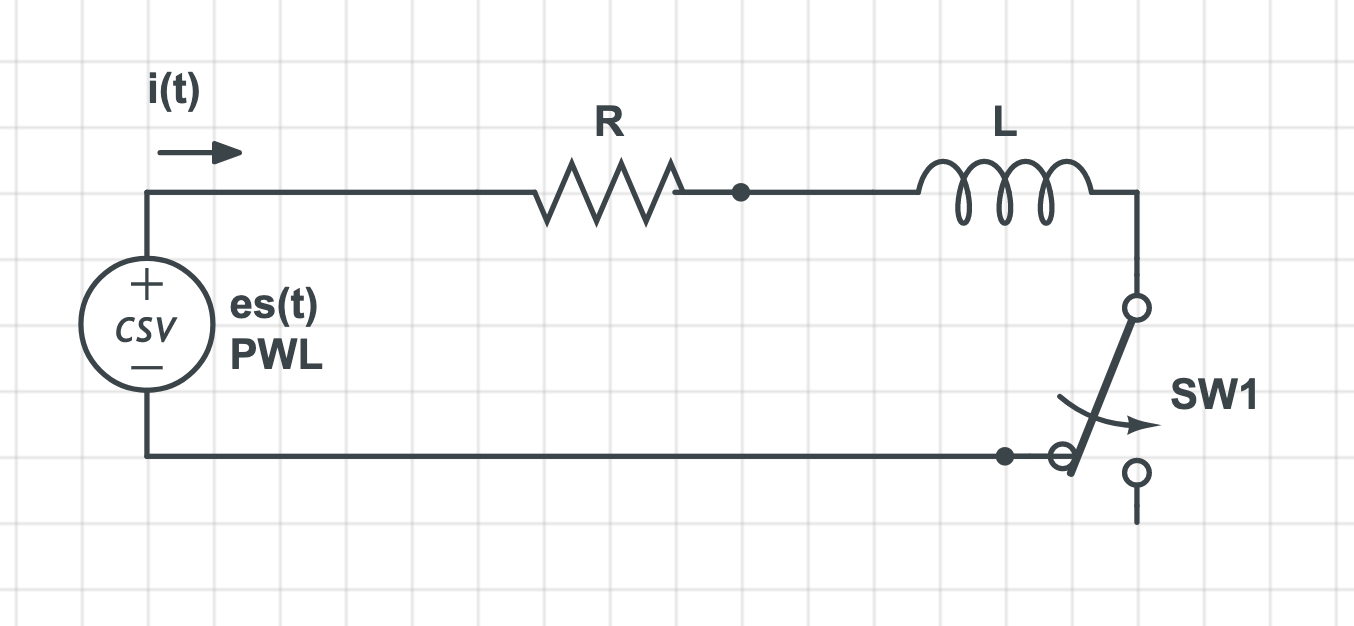
\includegraphics[width=1\linewidth]{img/transient1.png}
  %}
  \end{minipage}
  \hfill
  \begin{minipage}[c]{0.3\linewidth}
  % \subfloat{
    %}
  \end{minipage}  
  \label{transient1}
\end{figure}


\begin{subequations}
  \begin{equation}
    Ri + L \frac{di}{dt} = es(t)
  \end{equation}
  \begin{equation}
    i(t) = \frac{E}{R}[1 - e^{\frac{-t}{T}}]
  \end{equation}
  \begin{equation}
    T = \frac{L}{R}
  \end{equation}
\end{subequations}


When transforming the equation previously described in an algorithm, it is necessary to adopt discrete intervals of time $ \Delta t $, since digital computers are not able to simulate the idea of continuous-time. 

Assuming the single-phase case, \cite{dommel1969digital} describes the discrete representations for the inductors and the capacitor components, based on the trapezoidal numerical method integration:


\begin{figure}[H]
  \caption{Inductor - equivalent discrete representation}
  \centering
  \begin{minipage}[c]{0.59\linewidth}  
  %\subfloat{
    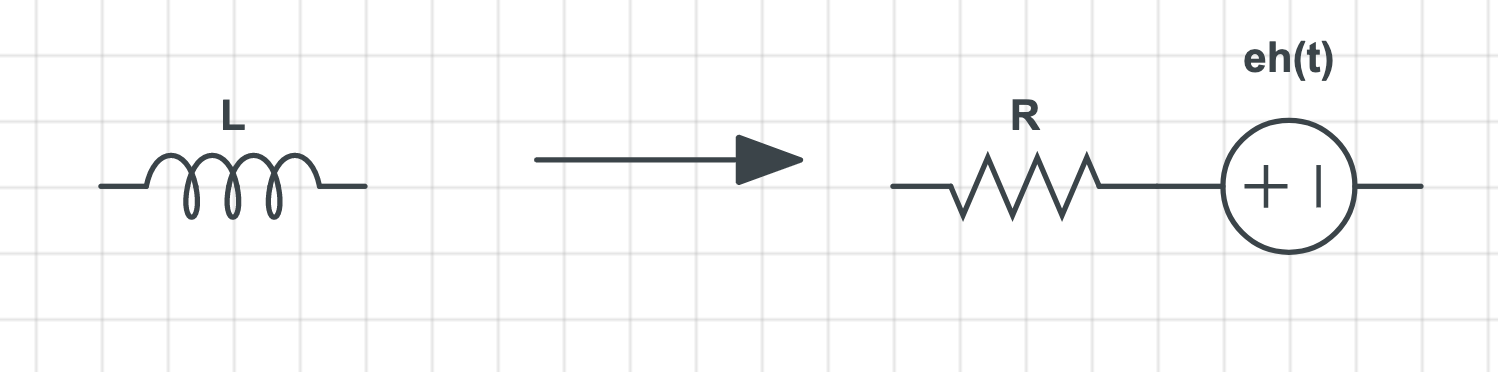
\includegraphics[width=1\linewidth]{img/Lequiv.png}
  %}
  \end{minipage}
  \hfill
  \begin{minipage}[c]{0.3\linewidth}
  % \subfloat{
    
    %}
  \end{minipage}  
  \label{transient2}
\end{figure}

\begin{subequations}
  \begin{equation}
    R = \frac{2 L}{\Delta t}
  \end{equation}
  \begin{equation}
    eh(t) = -V (t - \Delta t) - \frac{2 L}{\Delta t} i (t - \Delta t)
  \end{equation}
\end{subequations}


\begin{figure}[H]
  \caption{Capacitor - equivalent discrete representation}
  \centering
  \begin{minipage}[c]{0.59\linewidth}  
  %\subfloat{
    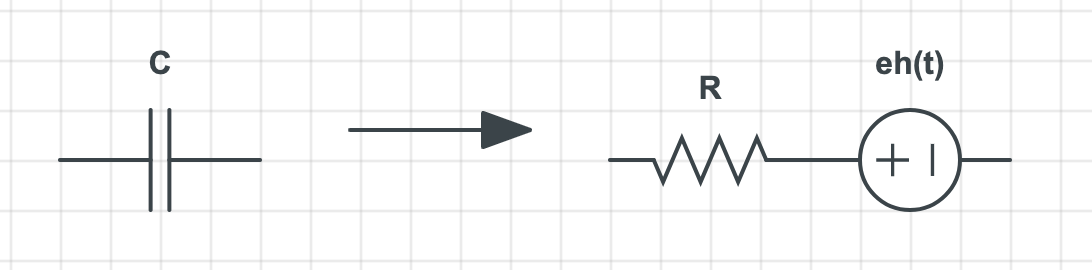
\includegraphics[width=1\linewidth]{img/Cequiv.png}
  %}
  \end{minipage}
  \hfill
  \begin{minipage}[c]{0.3\linewidth}
  % \subfloat{
    %}
  \end{minipage}  
  \label{transient3}
\end{figure}

\begin{subequations}
  \begin{equation}
    R = \frac{\Delta t}{2 C}
  \end{equation}
  \begin{equation}
    eh(t) = V (t - \Delta t) + \frac{\Delta t}{2 C} i (t - \Delta t)
  \end{equation}
\end{subequations}


Other numerical methods can be taken into consideration. Each distinct numerical method can generate different equivalent values for the limped L and C components. The trapezoidal integration method has been used in academic and commercial EMTP-based programs mainly due to its accuracy and stability properties. Analysing the advantages or disadvantages of each method is out of the scope of this work.

\section { EMTP algorithm }

Into EMTP or ATP software, the discrete models previously described compose a matrix equation in the following format:

\begin{figure}[htb]
  \caption{Nodal matrix model}
  \centering
  
  % \subfloat{
    \begin{subequations}
      \begin{equation}
        [G][V] = [h]
      \end{equation}
      % \begin{equation}
      %   eh(t) = V (t - \Delta t) + \frac{\Delta t}{2 C} i (t - \Delta t)
      % \end{equation}
    \end{subequations}
    %}
  \label{transient3}
\end{figure}

At \ref{transient3}, $ G $ is the matrix of conductances, $ V $ is the vector of unknown voltages and $ h $ is the vector of known current sources (independent current sources and the historical equivalent current sources).

It is possible to state a general algorithm \cite{dommel1969digital} in electromagnetic transients analysis according to the following procedures:
\begin{enumerate}
  \item Read the input data;
  \item Build the steady-state solution matrix;
  \item Build the transient solution matrix (G);
  \item Find the steady-state solution to initialise histories;
  \item Assume $ t = \Delta t $;
  \item \label{evaluateh} Evaluate current and voltage sources; 
  \item Solve for node voltages;
  \item Update history functions;
  \item Increment t: $ t = t + \Delta t $;
  \item Go back to item \ref{evaluateh} if the maximum simulation time hasn't been reached.
\end{enumerate}

\section{Existing commercial software}

In this section, an overview of the two major programs used for electromagnetic transient analysis is presented. Both are written in imperative languages (Fortran, C and C++). Imperative programming stands for a programming paradigm that uses statements which can change a program's state. Chapter \ref{fp} brings a detailed explanation of this matter.

\subsection{ATP}

Written mostly in Fortran language, the Alternative Transient Program (ATP) \cite{atpsite} became popular in the 1970s and 1980s. Originally, the user had to insert the circuit data in a card, as well as the simulation parameters, and then run the algorithm. The code is not open source, and even though it is possible to download the software for free, there are some restrictions on its license:. "Licensing to use ATP is free of all charge for all who have not engaged in EMTP commerce" \cite{atplic}. 

Modern versions of ATP support a rich GUI, named ATPDraw. See an example at Figure \ref{atpdraw}.

\begin{figure}[H]
   \centering
   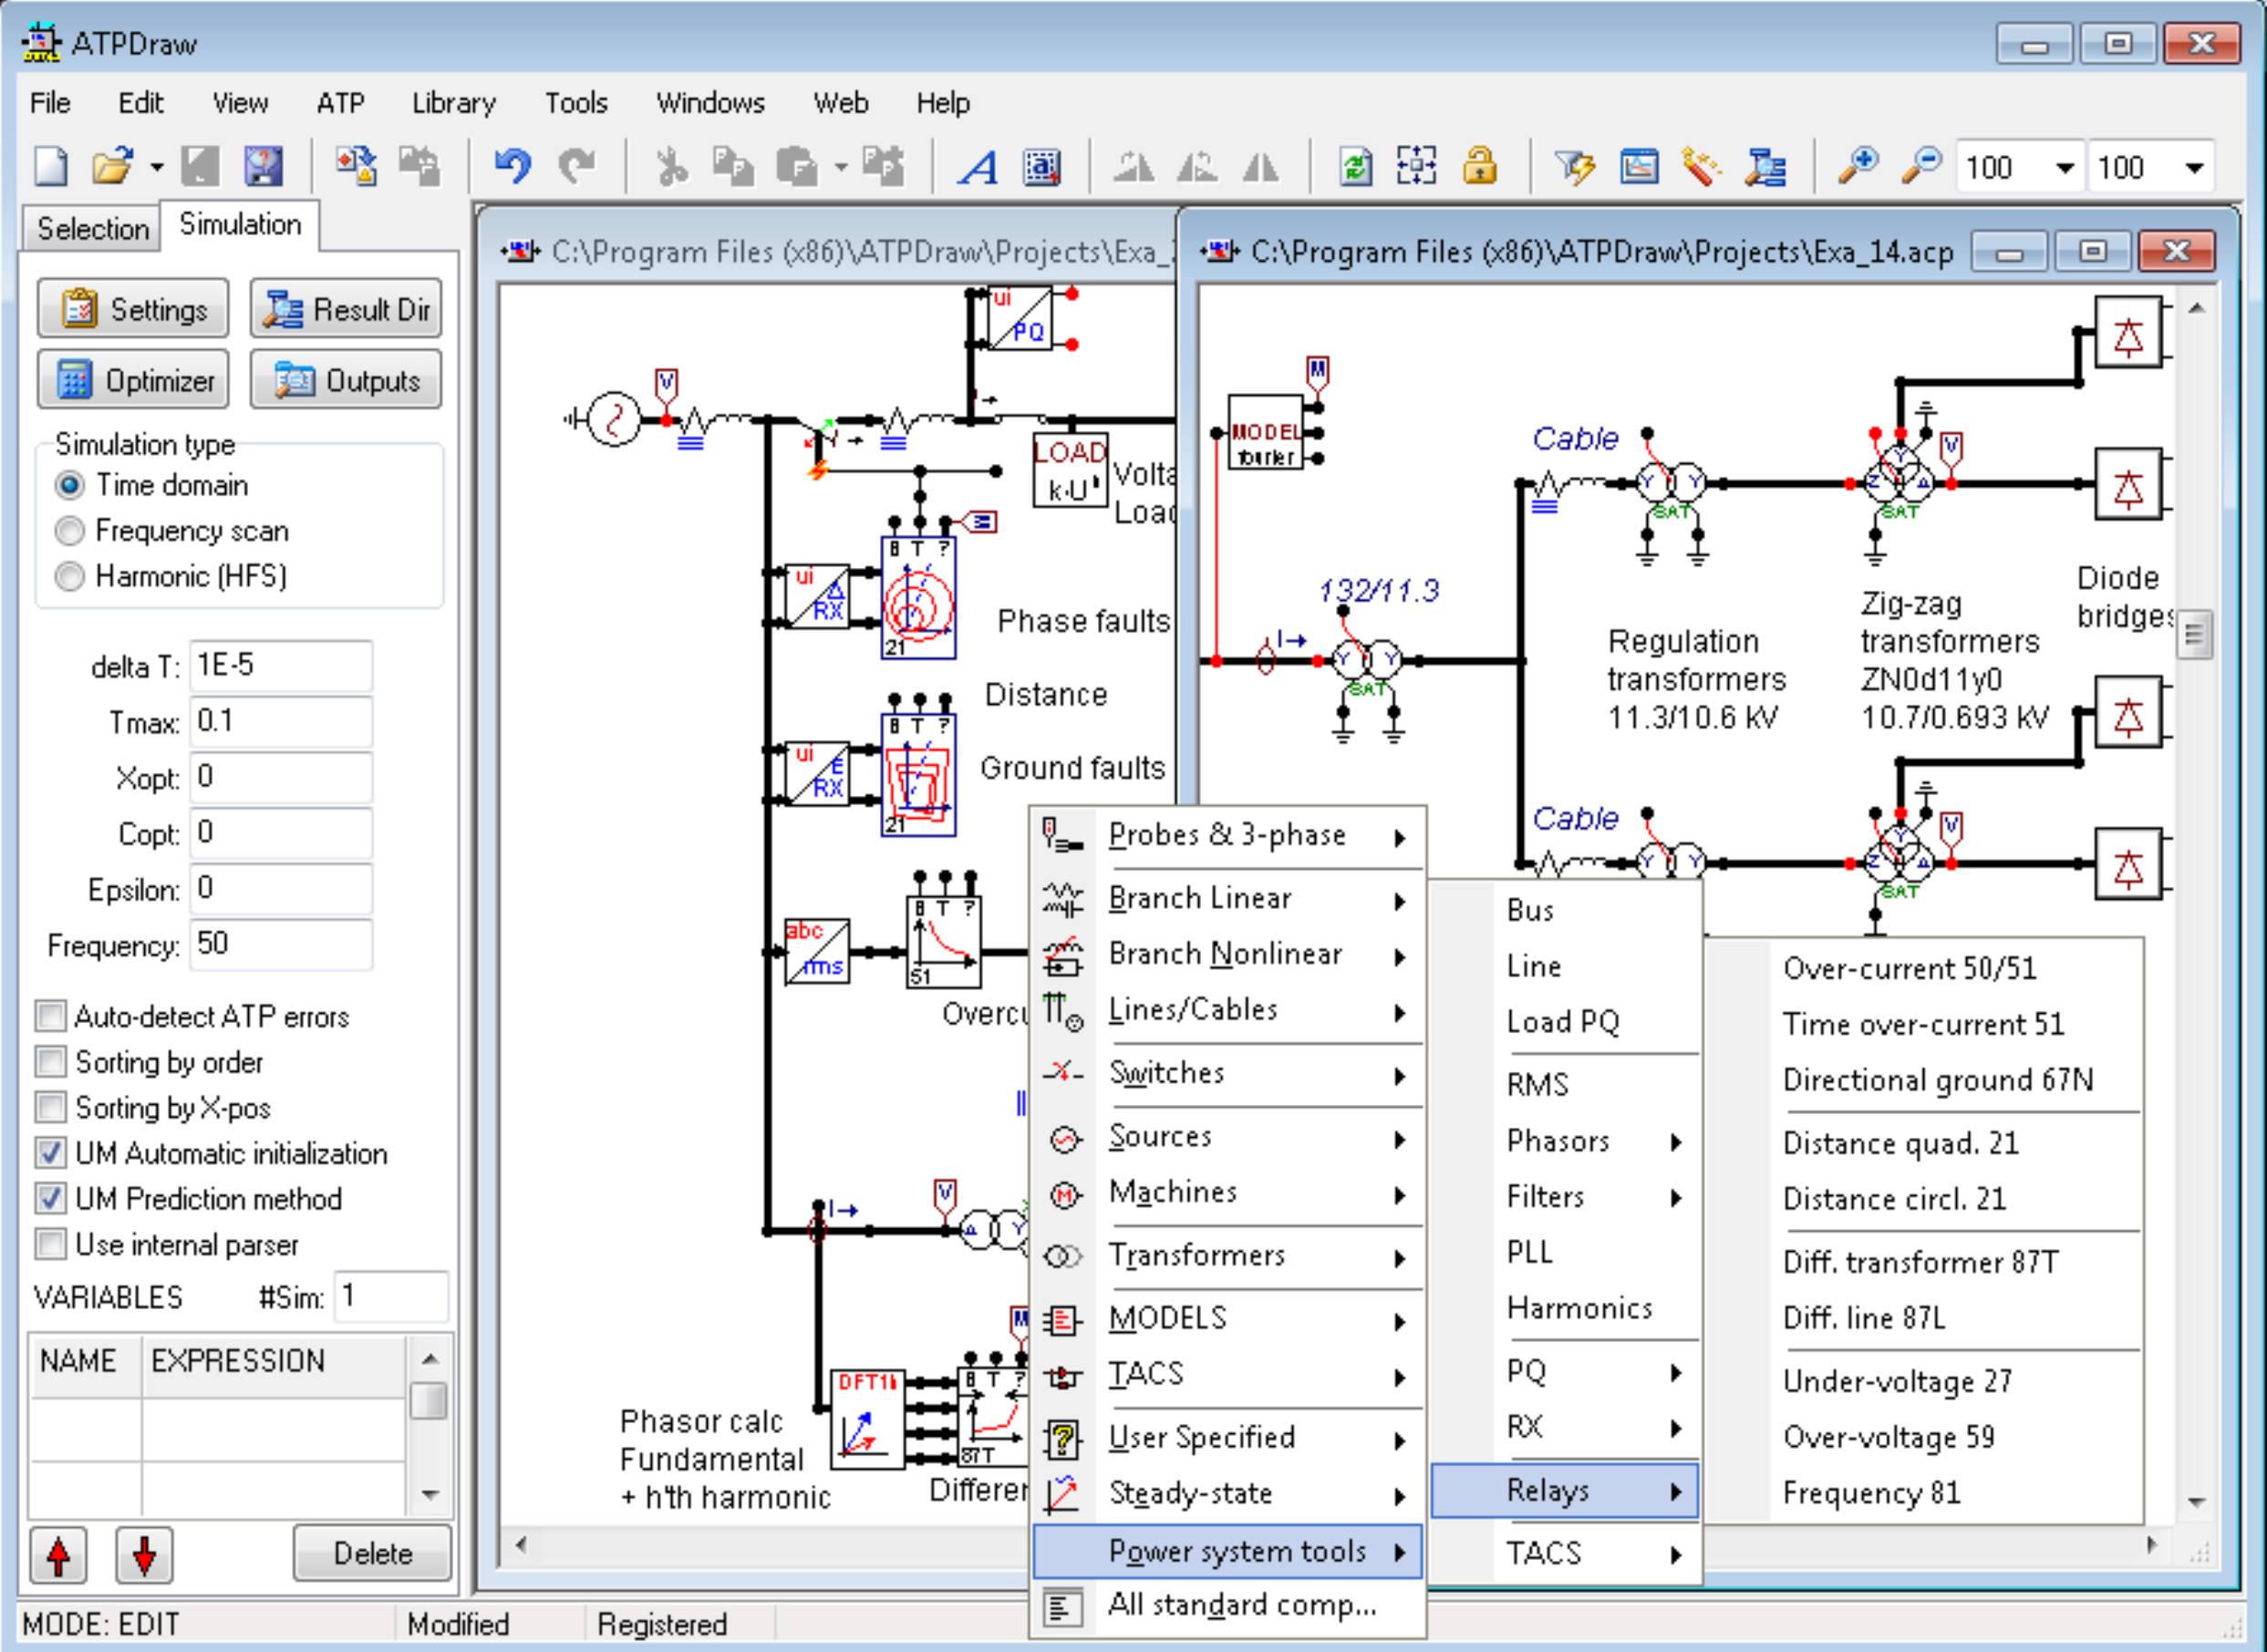
\includegraphics[width=0.8\textwidth]{img/atpdraw.png}
   \caption{ATPDraw}
   \label{atpdraw}
\end{figure}
\cite{atpsiteim}

ATP supports a wide variety of nonlinear components, switches, transformers and even support for the creation of customised elements. It can be used for time and frequency domain studies, lightning studies, electrical machines, control systems and power electronics projects.

\subsection{EMTP-RV}

EMTP-RV \cite{emtprv} is mostly written in C and C++. It was released on the market a few years after ATP. It is also a closed-source software, and it has a paid license. It is possible to obtain a free trial for a few days. It also comes with a sophisticated GUI, advanced machine models, transformer models which include magnetic core saturation and hysteresis, extensive library of control devices and functions and more.

\begin{figure}[H]
   \centering
   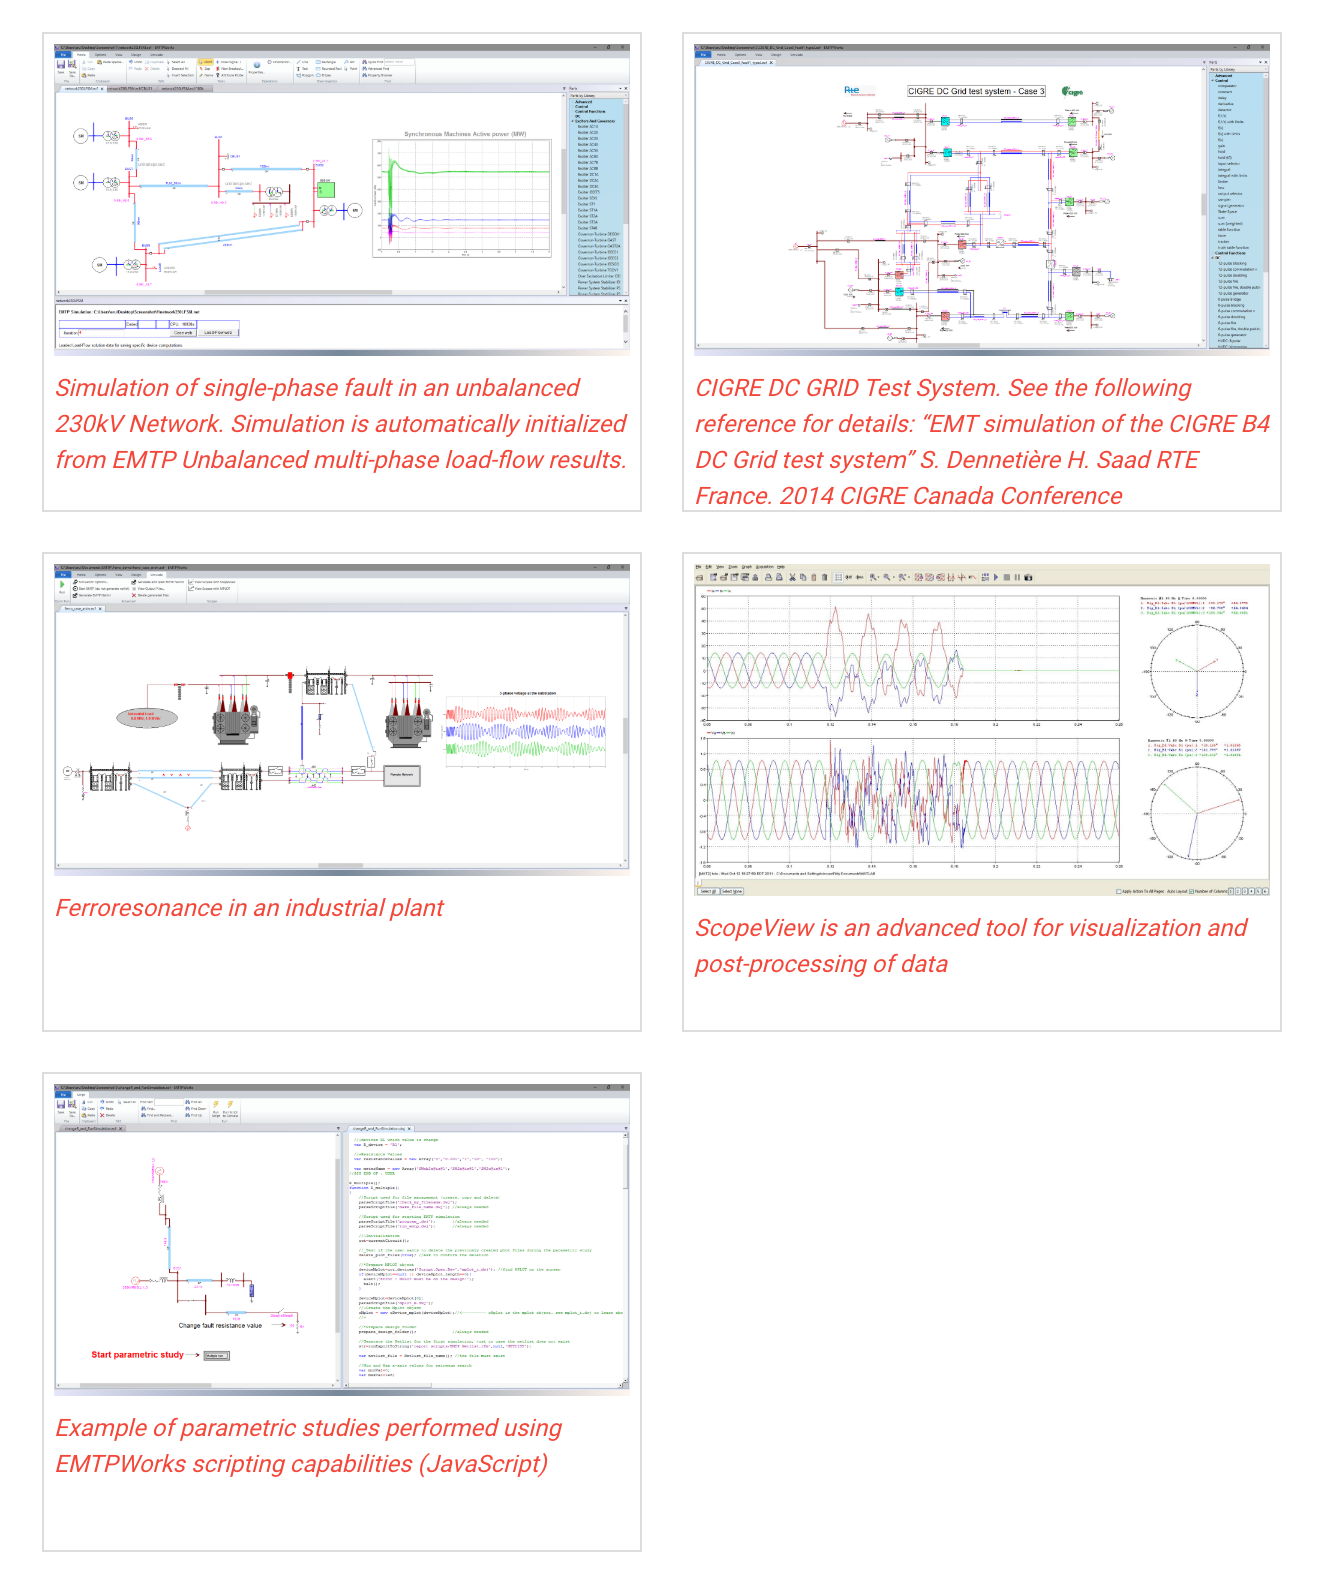
\includegraphics[width=0.8\textwidth]{img/emtp.png}
   \caption{EMTP}
   \label{emtp}
\end{figure}

EMTP implements, among other optimisations, the Critical Damping Adjustment (CDA) algorithm. "The CDA procedure eliminates the numerical oscillations that can occur in transients simulations that use the trapezoidal rule of integration"\cite{lin1990implementation}.

\section{Academic (didactic) software} \label{etr:academ}

Commercial versions are suitable for production projects, but for the learning process of undergraduate and graduate students, they might not be ideal, since their source code is often unavailable. Building a didactic prototype helps to understand the ideas behind the algorithms, possible optimisations and problems (numerical oscillations, errors, processing times). It also provides the students with a better understanding of the model and of the approach of nodal analysis method.

\subsection{ETR-P Matlab} \label{etr:thta}

Educational tool developed by a joint work from UNIFEI and UBC, this simplified Matlab/Octave version of an electromagnetic transient analysis program reads the user input from a file (in a similar format as ATP's cards) and executes the simulation. It can plot charts and it offers support to Transmission Lines, Switches and other nonlinear elements. Single-phase analysis only.

This academic project implements the CDA algorithm, as well as an equivalent technique  named by the authors of \cite{thta2015bonatto} as \textbf{"THTA"} - Trapezoidal History Term Averaging.

This project does not have an official name; the students refer to it simply as "THTA", but the nomenclature may lead to misinterpretation of what is the academic tool and what is, in fact, the Trapezoidal History Term Averaging optimisation. For this particular reason, this work refers to UNIFEI's implementation as \textbf{ETR-P} (Electromagnetic Transient Program).

ETR-P's source code is open, and it is possible to find it on Github \cite{thtaoctave}. It is not actively maintained and the code is purely procedural and imperative. It is restricted to the Matlab/Octave environment.

\subsection{ETR-Py - Python} \label{etr:pythta}

Inspired by ETRP-P, ETR-Py \cite{tavante2018open} implements a subset of features from ETR-P using the Python Language, this time using Object Oriented programming, classes, modules and popular libraries such as NumPy and SciPy. The code is also available at Github - \cite{pythta}. The features for chart plotting, Transmission Lines and Switches are not implemented yet.

When this Python version was proposed, it used to be called "PyTHTA". Once again, to avoid misunderstandings with the term "THTA", this work replaces the former name with \textbf{ETR-Py}.


\subsection{Comparison of the software alternatives}

Up to this point, only imperative code has been used to build a program to run an electromagnetic transient analysis simulation. There are other programming paradigms, and this work adopts one of them (\textbf{Functional Programming}) to create a new version of ETR-P using an utterly distinct programming style. The elaboration of this other program, named \textbf{Haskell ETR-P}, will make a robust comparison between advantages and disadvantages of each programming style possible. The code is also be open source and it is already on Github \cite{thtahs}.

The Haskell version of ETR-P aims to provide a solution where students can focus on the algorithm itself, and not on the "language plumbing" (particularities of a programming language that are required to make a program work properly but demand time and expertise to get it right). The existing academic versions mentioned at \ref{etr:thta} and even the more recent \ref{etr:pythta} are subjected to the existing problems of the imperative programming paradigm. The new approach with functional programming may help the students to use more time thinking about the algorithm and new ways to improve it.






